\documentclass{article}

%Headers
\usepackage[dvips]{graphicx}    %package that does pdfs
\usepackage{color}              %this needs to be here also
\usepackage[T2A]{fontenc}
\usepackage[utf8]{inputenc}
\usepackage{listings}
\usepackage{float}
\usepackage{authblk}



\lstdefinestyle{pythonstyle}{
  language=Python,
  basicstyle=\small\ttfamily,
  keywordstyle=\color{blue},
  commentstyle=\color{green},
  stringstyle=\color{black},
  showstringspaces=false,
  tabsize=4,
  frame=single,
  numbers=left,
  numberstyle=\tiny\color{black},
  stepnumber=1,
  numbersep=8pt,
  firstnumber=1,
  breaklines=true,
  xleftmargin=15pt,
  framexleftmargin=15pt,
  backgroundcolor=\color{white},
  captionpos=b
}



\title{Практическая работа по дисциплине "Нейроэволюционные вычисления"}
\author{Выполнил: Малкин Артем Юрьевич\\ Студент гр. 8ВМ22 \and Проверил: Григорьев Дмитрий Сергеевич\\ Старший преподаватель ОИТ ИШИТР ТПУ}



\date{19 Мая 2023}

\begin{document}
\maketitle

%Note that the '*' surpresses the section numbering
\section*{Номенклатура}
\label{sec:nomenclature}
\begin{tabbing}
    XXXXXXXX \= \kill% this line sets tab stop
	NEAT				\> NeuroEvolution of Augmenting Topology\\  
	IoU					\> Intersection over Union\\    
	CUDA				\> Compute Unified Device Architecture\= \kill    
	IN 					\> Innovation Number 
\end{tabbing}

\section*{Цель работы}
Реализовать алгоритм NEAT для решения задачи определения людей, больных диабетом, по данным анализов. 

\section{Ход работы}
\subsection{Используемые программные модули}

В рамках практической работы был разработан программный код с применением модуля neat-python для реализации нейроэволюционного алгоритма NEAT. Для отображения схемы получившейся нейронной сети используется модуль networkx (создание объектов для дальнейшего их отображения) и matplotlib. \\

Модуль pandas используется для загрузки данных о людях, больных диабетом. Датасет представлен на сайте Kaggle\cite{Kaggle_dataset}. Программный код был разработан на языке Python.


\subsection{Описание алгоритма NEAT}
Алгоритм NEAT предназначен для поиска оптимальной структуры нейронной сети, которая разрешит поставленную задачу. К примеру, задача определения людей, больных диабетом или раком, на основании анализов. Поиск оптимальной структуры нейронной сети предполагает поиск: 

\begin{itemize}
    \item Оптимального количества нейронов в скрытом слое сети, определение их связей.
    \item Оптимальных весовых коэффициентов для связей между нейронами.
\end{itemize}

Алгоритм NEAT оперирует инновационными числами (Innovation Numbers - IN), который содержит информацию о связях между нейронами, их весовом коэффициенте и включена ли эта связь. На рисунке ~\ref{fig:Neat1} (взят из оригинальной статьи создателя алгоритма Kenneth O. Stanley \cite{Stanley_NEAT}) сверху показан пример мутации нейронной сети: добавлена связь от нейрона 3 к нейрону 5. Поскольку такой связи ранее не было, этой информации о связи присваивается очередное IN. Если в ходе мутации создалась бы связь, которая уже участвовала в нейроэволюционном алгоритме, только что созданная связь получит то же IN.

На том же рисунке снизу при создании нового узла (Node) определились связи от нейрона 3 к нейрону 6 и от 6 к 4. Поскольку ранее была связь от 3 и 5 (IN = 7), а сейчас его нет, то данный представитель популяции лишается в своём фенотипе  информации о этой связи.

%Illustrate inserting a figure
\begin{figure}[h]
	\centering
    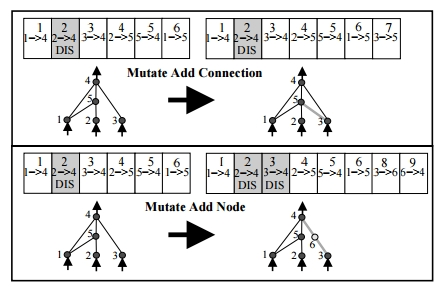
\includegraphics[width=3in]{neat1}
    \caption{Процесс мутации нейронной сети }
    \label{fig:Neat1}
\end{figure}

До того, как начать мутации, необходимо создать популяцию особей, а также произвести отбор особей. Оценка того, насколько особь приспособлена к решению поставленной задачи, происходит по заданной пользователем функции (fitness function). Те особи, что более близки к требуемым значениям (этап селекции), имеют больше шансов на скрещивание.

Скрещивание происходит по трём действиям:
\begin{enumerate}
    \item Сопоставление генов. Гены - связи между узлами (нейронами) в сети. Совпадающие гены - те, которые имеют одинаковые IN, указывающие на происхождение генов. Совпадающие гены наследуются случайным образом от одного из родителей потомству.
    \item Несовпадающие и избыточные гены. Несовпадающие - те, у которых различные IN и они находятся в одинаковом положении в геноме. Избыточные гены - гены с инновационным числом, превышающим число генов другого родителя. Оба типа генов наследуются от более приспособленного родителя без изменений.
    Если IN у генов совпадает, но различны состояния активности (enable/disable), то используется элемент случайности, согласно которой с некоторой долей вероятности потомок получит активированный или неактивированный ген. Это состояние может измениться в процессе мутации.
    \item Весовые коэффициенты связей. После определения структурных генов устанавливаются веса связей между генами потомства. Одним из методов является усреднение весов связей совпадающих генов обоих родителей. 
\end{enumerate}

На рисунке ~\ref{fig:Neat2} продемонстрирован пример операции кроссовера (скрещивания) особей для создания потомства.

%Illustrate inserting a figure
\begin{figure}[h]
	\centering
    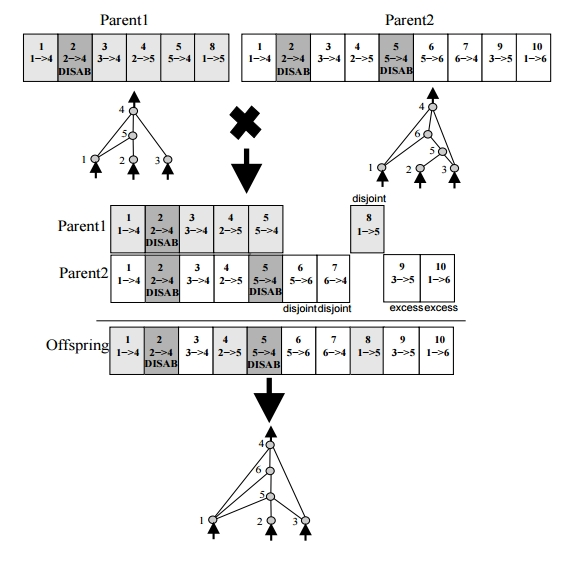
\includegraphics[width=3in]{neat2}
    \caption{Операция кроссовера особей}
    \label{fig:Neat2}
\end{figure}

Вместо того, что огульно тратить пули, пытаясь случайно попасть в оптимальную структуру сети, можно использовать хитрый алгоритм NEAT. Пули не работают, Жон (рисунок ~\ref{fig:Jon}).

\begin{figure}[h]
	\centering
    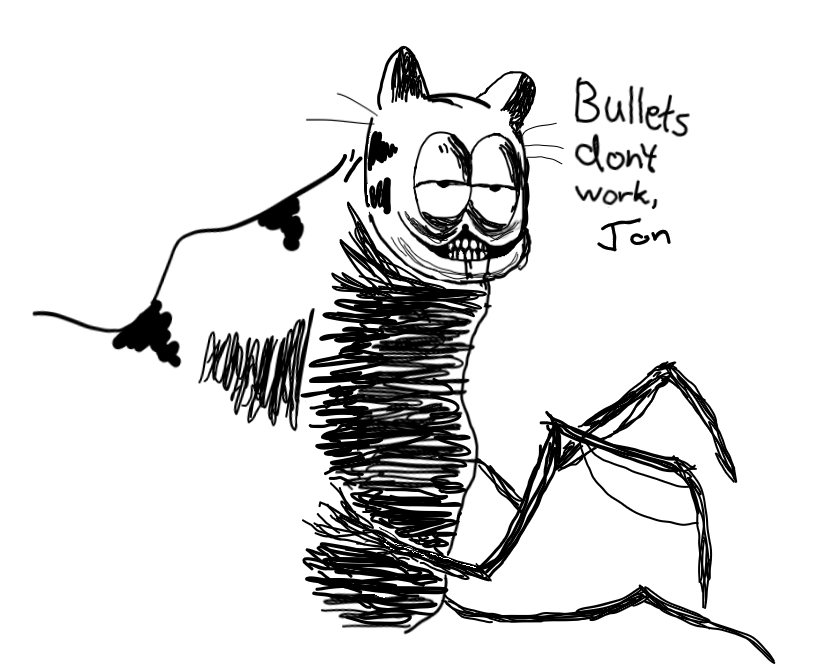
\includegraphics[width=3in]{jon1}
    \caption{Bullets don't work, Jon}
    \label{fig:Jon}
\end{figure}

Вот так.


%Illustrate breaking the document into several .tex files and then including them together with 'input'
\section{Программный код}
В рамках данной работы был разработан программный код с применением модуля neat-python для реализации нейроэволюционного алгоритма NEAT. Программный код был разработан на языке Python.

% add program code abd color it
\begin{lstlisting}[style=pythonstyle, caption={Программный код реализации алгоритма NEAT с применением модуля neat-python}, label={lst:pythoncode}]
import networkx as nx
import matplotlib.pyplot as plt
import matplotlib.patches as mpatches
import pandas as pd
import neat
import my_visualize as visualize
import numpy as np
import pickle

dataset = pd.read_csv('diabetes.csv', header=None, sep=',', engine='python')
dataset = dataset.drop([0])
dataset = dataset.astype(float)
inputs = dataset.iloc[:, 0:8].values
outputs = dataset.iloc[:, 8].values
inputs = np.array(inputs)
outputs = np.array(outputs)
config_path = 'config-diabetis'
config = neat.Config(neat.DefaultGenome, neat.DefaultReproduction,
                         neat.DefaultSpeciesSet, neat.DefaultStagnation,
                         config_path)

def eval_genomes(genomes,config):
    '''
    evaluate genomes
    '''
    for genome_id, genome in genomes:
        genome.fitness = len(inputs)
        net = neat.nn.FeedForwardNetwork.create(genome, config)
        for xi, xo in zip(inputs, outputs):
            output = net.activate(xi)
            #use threshold
            output = 1 if output[0] > 0.5 else 0
            genome.fitness -= (output - xo) ** 2

def plot_the_graph(winner):
    '''
    plot the graph of the winner
    '''
    list_of_nodes = []
    for node in winner.connections.values():
        temp = []
        for neuron in node.key:
            temp.append(neuron)
        temp.append(node.weight)
        list_of_nodes.append(temp)
    
    unique_nodes = []
    for node in list_of_nodes:
        if node[0] not in unique_nodes:
            unique_nodes.append(node[0])
        if node[1] not in unique_nodes:
            unique_nodes.append(node[1])
    
    G = nx.DiGraph()
    i_neg = 0
    i_pos = 0
    for node in unique_nodes:
        if node > 0:
            G.add_node(node, pos=(1, i_pos ))
            i_pos += 2
        elif node < 0:
            G.add_node(node, pos=(0, i_neg))
            i_neg += 2
        else:
            G.add_node(node, pos=(2, 5))

    for node in list_of_nodes:
        G.add_edge(node[0], node[1], weight=node[2])

    # positions of the nodes
    pos = nx.get_node_attributes(G, 'pos')

    # color the arrows
    edge_colors = ['r' if G[u][v]['weight'] < 0 else 'g' for u,v in G.edges()]
    # green for input nodes, yellow for hidden nodes, red for output nodes
    node_colors = ['gray' if node < 0 else 'y' if node > 0 else 'pink' for node in G.nodes()]

    # add legend to plot
    red_patch = mpatches.Patch(color='red', label='Negative weights')
    green_patch = mpatches.Patch(color='green', label='Positive weights')
    gray_patch = mpatches.Patch(color='gray', label='Input nodes')
    yellow_patch = mpatches.Patch(color='yellow', label='Hidden nodes')
    pink_patch = mpatches.Patch(color='pink', label='Output nodes')

    plt.legend(handles=[red_patch, green_patch, gray_patch, yellow_patch, pink_patch])

    # weights of the edges
    weights = nx.get_edge_attributes(G, 'weight')
    # draw the graph
    nx.draw(G, pos, with_labels=True, node_color=node_colors, edge_color=edge_colors, node_size=500, arrows=True)
    # draw the weights
    #nx.draw_networkx_edge_labels(G, pos, edge_labels=weights)
    plt.show()

def calculate_metrics(winner_net, inputs, outputs):
    '''
    calculate metrics for winner net    
    '''
    TP = 0
    TN = 0
    FP = 0
    FN = 0
    for xi, xo in zip(inputs, outputs):
        output = winner_net.activate(xi)
        output = 1 if output[0] > 0.5 else 0
        #print("input {!r}, expected output {!r}, got {!r}".format(xi, xo, output))    
        if output == 1 and xo == 1:
            TP += 1
        elif output == 0 and xo == 0:
            TN += 1
        elif output == 1 and xo == 0:
            FP += 1
        elif output == 0 and xo == 1:
            FN += 1

    accuracy = (TP + TN) / (TP + TN + FP + FN)
    precision = TP / (TP + FP)
    IoU = TP / (TP + FP + FN)

    print("TP: ", TP)
    print("TN: ", TN)
    print("FP: ", FP)
    print("FN: ", FN)
    print("accuracy: ", accuracy)
    print("precision: ", precision)
    print("IoU: ", IoU)

def launch(generations = 300, reporter = False, checkpoint = False):
    '''
    launch NEAT algorithm
    '''
    p = neat.Population(config)
    # Add a stdout reporter to show progress in the terminal.
    if (reporter):
        p.add_reporter(neat.StdOutReporter(True))
    stats = neat.StatisticsReporter()
    p.add_reporter(stats)
    if (checkpoint):
        p.add_reporter(neat.Checkpointer(5))
    winner = p.run(eval_genomes, 300)
    # Display the winning genome.
    print('Best genome:\n{!s}'.format(winner))
    winner_net = neat.nn.FeedForwardNetwork.create(winner, config)
    calculate_metrics(winner_net, inputs, outputs)
    #visualize.draw_net(config, winner, True, node_names=node_names)
    visualize.plot_stats(stats, ylog=False, view=True)
    return winner

def save_model(model, path):
    '''
    save model using pickle
    '''
    with open(path, 'wb') as output:
        pickle.dump(model, output, pickle.HIGHEST_PROTOCOL)

def load_model(path):
    '''
    load model using pickle
    '''
    with open(path, 'rb') as input:
        model = pickle.load(input)
    return model
        
    
        
\end{lstlisting}

\section{Результаты работы}

В датасете содержится 784 записей о людях, которые могут быть больны диабетом. В результате работы нейроэволюционного алгоритма NEAT в количестве 300 поколений была получена модель, значение фитнес-функции которой составляет 541 (то есть из 784 данных записей она правильно предскажет наличие или отсутствие болезни в 541 случае).

Был получен словарь (Python Dictionary), содержащий информацию о связях между нейронами входного, скрытого, выходного слоёв. Информация (рисунок ~\ref{fig:Output3}) включает в себя сведения о:

\begin{itemize}
    \item Скрытых и выходном нейронах: смещение, функция активации, способ агрегации.
    \item Связях между нейронами: входной и выходной нейроны, весовой коэффициент, активирована ли связь.
\end{itemize}

\begin{figure}[h]
	\centering
    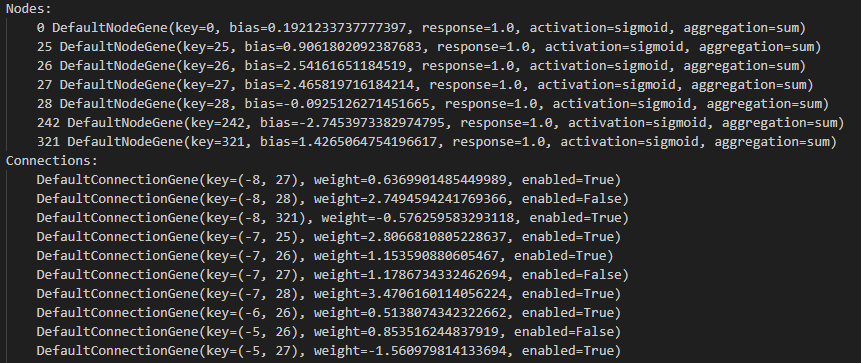
\includegraphics[width=4in]{output3}
    \caption{Выходные данные о лучшей модели (в отчёте приведён неполный список Connections)}
    \label{fig:Output3}
\end{figure}

Была проведена оценка качества предсказания метриками Accuracy и Precision, IoU. Были определены следующие значения TP, TN, FP, FN:

\begin{itemize}
    \item TP: 83 (столько человек действительно болеют диабетом, модель корректно их определила как больных людей).
    \item TN: 458 (человек не болеет, система полагает так же).
    \item FP: 42 (человек не болеет диабетом, но модель считает иначе).
    \item FN: 185 (человек болеют диабетом, но система не опредилила их).    
\end{itemize}

Таким образом, значение метрики Accuracy составляет 0.7044, Precision - 0.664, IoU - 0.2677. Эти метрики говорят о не лучшем определении людей, больных диабетом, как людей, которые болеют диабетом. Но модель показывает хорошие результаты, когда нужно подтвердить, что человек не болен диабетом.

На рисунке ~\ref{fig:Output1} представлен график значений фитнес-функции у лучшей модели и в среднем по поколению (с учётом стандартного отклонения).

\begin{figure}[h]
	\centering
    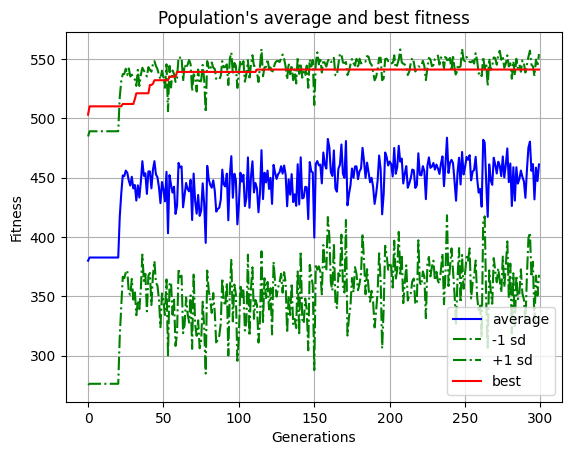
\includegraphics[width=3in]{output1}
    \caption{Среднее и лучшее значения фитнес-функции у популяции}
    \label{fig:Output1}
\end{figure}

На рисунке ~\ref{fig:Output2} представлена cхема нейронной сети лучшей модели. На рисунке цифрами [-8:0] обозначены:
\begin{itemize}
    \item 0: выходной сигнал (1 или 0 - болен или здоров)
    \item -1: Pregnancies - количество беременностей
    \item -2: Glucose - концентрация глюкозы в плазме через 2 часа после пероральной нагрузки
    \item -3: BloodPressure - диастолическое артериальное давление (мм рт. ст.)
    \item -4: SkinThickness - толщина кожной складки (мм)
    \item -5: Insulin - 2-часовой сывороточный инсулин (мкЕд/мл)
    \item -6: BMI - индекс массы тела (масса в кг / (рост в м)**2)
    \item -7: DiabetesPedigreeFunction - функция родословной диабета
    \item -8: Age - возраст (полных лет)
\end{itemize}

\begin{figure}[h]
	\centering
    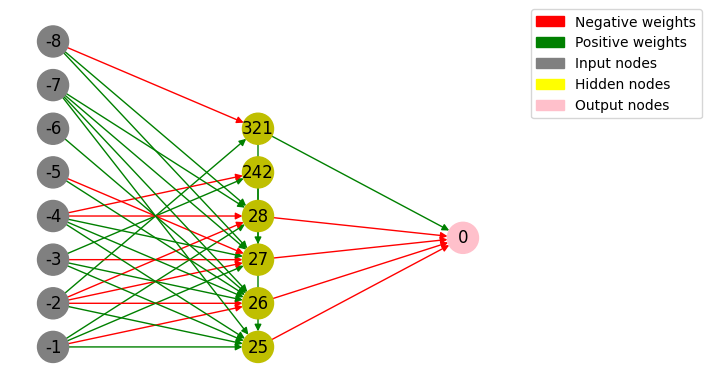
\includegraphics[width=3in]{output2}
    \caption{Структура лучшей модели}
    \label{fig:Output2}
\end{figure}

Для оценки промежуточного результата есть возможность изучать значения фитнес-функции есть встроенный в neat-python инструментарий (рисунок ~\ref{fig:Output4}).

\begin{figure}[h]
	\centering
    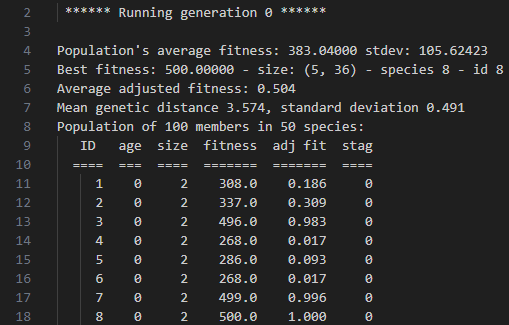
\includegraphics[width=3in]{output4}
    \caption{Оценка фитнес-функции у особей данного поколения}
    \label{fig:Output4}
\end{figure}

\section*{Заключение}
В ходе выполнения практической работы было получение представление работы алгоритма NEAT в задачах поиска оптимальной структуры нейронной сети. Разработан программный код с применением модуля neat-python для реализации данного алгоритма на языке высокого уровня Python. Реализована функция отображения структуры нейронной сети, полученной в результате работы алгоритма NEAT. Получен опыт работы с набором макрорасширений системы компьютерной вёрстки TeX.

%Illustrate creating a bibliography by referring to an external bibliography file (SampleBibliography.bib).  Note that you must chose a style to determine how the bibliography is presented
\bibliography{SampleBibliography}
\bibliographystyle{aiaa}

\end{document}
